% Chapter 3

\chapter{System Design} % Chapter title

% For referencing the chapter elsewhere, use \autoref{ch:design}
\label{ch:design}  

%TC:ignore
%This is the System Design chapter, should be approximately 4,000 Words in total.
%The PUF section should be approximately 1,250 words long.
%The main Fuzzy Extractor section should be approximately 1,250 words long
%Cryptographic Hashing section, it should 750 words long.
%Networking section should be 750 words in length.
%TC:endignore
%-------------------------------------------------------------------------------


\section{Introduction}

Ideally a complete \gls{puf}-based authenticatable device could be implemented
on a single \gls{fpga}, containing all the necessary components required.
However, given the time constraints of a Masters project, while this approach
was initially favoured, it was deemed necessary to simulate parts of the system
in the \matlab programming environment. The system area considered most
difficult to synthesise was the error correction encoder and decoder, without
which a Fuzzy Extractor could not be implemented, thus both the generator and
reproduction implementations of the Fuzzy Extractor in it's
entirety were not implemented in \gls{fpga}.

The Ethernet protocol is also comparatively complex and so modification of this
for the purposes of devices authentication was also removed from the design.
Instead a study of possible protocol schemes was made with
a simulation of only one message of the complete scheme developed to a level
for demonstration.

The \gls{puf} functionality of \gls{sram} on the other hand is something
that was felt possible for full implementation in \gls{fpga}, due to the easy availability of multiple DE-1 development boards, each with integrated
\gls{sram} chips.
To extract specific \gls{puf} data from the \gls{sram} chip would require the design of
a 'wrapper' function that could issue memory addresses and retrieve memory
contents of the \gls{sram} chip. It would then be necessary to link that wrapper
with a communication system that would allow external access of the device.

It was decided to implement this system using the RS-232 protocol standard. 
This is because the necessary hardware was available on the DE-1 board and it was
deemed the most simple to implement.
The development of a UART that could receive memory address locations encoded
serially and pass them in full to the wrapper was thus required.
Likewise it would be necessary to send the memory contents passed from the 
wrapper serially back to the requester.
This requester would be a full PC running \matlab which contains
the ability to integrate serial communications data into it's programs.

\section{SRAM-PUF interface implementation on FPGA}

\subsection{SRAM}

The DE-1 Development Board contains a IS61LV25616 chip. This is contains
$2^{22}$ SRAM cells organised into $2^{18}$ words of 16-bits each. This
should be a more than sufficient quantity of memory for testing our design.
In fact, for the purposes of simplicity, it is easier to use only a quarter
of the address space the chip provides, to allow 16-bit addressing which
reduces the complexity of the communications (via RS-232) part.
To access the chip as a \gls{puf} we need only to concern ourselves with
the read cycle of the device. There are 5 control lines to the chip (all
use active-low);
Chip Enable ($\overline{CE}$),
Write Enable ($\overline{WE}$),
Output Enable ($\overline{OE}$),
Lower Byte Access ($\overline{LB}$) and
Upper Byte Access ($\overline{UB}$).
While the first three can remain in a constant state for our purposes
($\overline{CE} = 0, \overline{WE} = 1, \overline{OE} = 0$), the byte access signals
can be utilised to output the full 16-bit memory data onto just one 8-bit bus
by cross-wiring the low order bits lines (0-7) to the high order bits (8-15)
sequentially.
Therefore a full reading can be sent via the rs-232 link in two transmissions.
In a similar way the 16-bit address will be received in two pieces.
Timing is important, and the particular chip on the development board is the 
fastest in the range with an access time of 10ns rather than 12ns or 15ns in
other chips in the family.
Thus, with careful reading of the datasheets\cite{sramdatasheet}, from
the initial setting of the address to the point at which the data output is
valid\footnote{$t_{AA}$, or Address Access Time} is 10ns.

It can be seen that a wrapper function is required that buffers the two part address
as it is received then 'forwards' a complete 16-bit address onwards to 
the address bus of the \gls{sram} memory, with the Upper Byte Access signal active.
After some delay greater than 10ns the upper byte can be 'forwarded' and the
Upper and Lower Byte Access signals toggled. After at least another identical delay
and if a strobe has been recieved from the communication module to say the previous
byte has been sent the lower byte can be forwarded. Thus ew have a system for
converting challenges in the form of memory addreses into responses in the form of
memory data. 

\subsection{UART Implementation}

The DE-1 Development Board contains a MAX232 chip that can handle the 
conversion of on-board logic levels to the higher voltages required by the
RS-232 standard, so this was not required to be implemented manually.
Instead the timing requirements of the protocol needed to be met.

A Universal Asynchronous Receiver/Transmitter (abbreviated UART) provides
serial communication between devices. In essence the UART controls the process
of converting data arriving from a parallel data bus into a form that can
be sent sequentially (one bit at a time) over a communication channel.

A fundamental component of a UART is the Shift Register. In the case of 
reception a Serial-In, Parallel-Out (SIPO) Shift Register is used.
Similarly, in the case of transmission a Parallel-In, Serial-Out (PISO)
type is required.

Synchronisation of the rate at which the bits are sent (Baud) is critical.
While clock skew is not an issue as there is no master clock, data recovery
still depends on both devices being set to operate at the same speed.
Common bit rates supported range from 75 to 115,200 bits/s.

The RS-232 protocol uses binary signalling. When idle the channel is left at
a logical high.
Data send is framed by sending an initial low start bit and ended with a
high stop bit. The stop 'bit' isn't really a bit a all, just the convention
that the channel returns to a logical high for at least one clock cycle
after the transmittion of data.
It can therefore be specified 1.5 or 2 'bits' in length, but this is unusual).
The data itself can have a data word length of 5 to 9 bits, but is usually
8 (1 byte) and an optional parity bit (Even, Mark or Space parity) 
can be appended.

Our implementation will fix on just one possibility for all these values,
in the common shorthand, we use '115200/8-N-1', meaning that
the baud is 115,200 bits per second, there are 8 data bits, no parity bits
and 1 stop bit. <<TODO ADD DIAGRAM OF RS-232 PROTOCOL>>
While RS-232 can utilise extra handshaking signals, for flow control,
however these are not required and so are not implemented.

The design of a \gls{uart} is split into two distinct halves; the transmitter
and the receiver. Each operates somewhat independantly. 

\subsubsection{Transmitter}

The PISO Shift Register is a component of this half of the UART.
Transmission

\subsubsection{Receiver}

\section{Fuzzy Extractor in MATLAB}

\subsection{Introduction}

The fuzzy extractor has two procedures, the Generation procedure and the
Reproduction procedure.
The generation procedure is only used for initial set-up, whereby the expected
Responses for all possible Challenges are generated and securely stored.
This process is likely to happen during manufacturing of the device at the
factory.
The Reproduction procedure on the other hand, is the commonly employed procedure
whereby for a given Challenge a Response is generated that can be tested against
the initial response from the Generation procedure. 
These are different because in the generation procedure, a response and helper
data must be generated.
Whereas, in the reproduction procedure, that previously generated helper data is
now required to allow for later differences in the raw responses of the \gls{puf}. 
In both cases, a randomness extractor consisting of a cryptographic hash
function is used to generate a Privacy Amplified response. In generation, raw
input from the \gls{puf} and random data is captured from a true random number
generator of the same length are combined through an XOR operator before being
applied as the input to an implementation of the SHA-256 cryptographic hash
function which outputs the response. In reproduction the input to the randomness
extractor needs to be generated through the secure sketch first but is still
applied to the hash function to output a response. The random data used must
also be stored unaltered as the first of two pieces of helper data
(let us call this ‘x’).

The core difference between the procedures occurs in the secure sketch process.
In generation, a ‘sketch’ is made and the required response is recorded. This
‘sketch’ results in helper data to be used in the reproduction procedure and is
stored in such a way that it can be sent with all challenges used in the
challenge-response protocol. In reproduction, a ‘recovery’ is performed,
whereby the previously generated helper data and the noisy input from the \gls{puf}
are processed to produce an input for the randomness extractor.

More accurately, the ‘sketch’ takes in two inputs; the first is the raw data
from the \gls{puf} that is known to be noisy and the second is random data generated
by the first of two independent true random number generators (we shall name
this the ‘Sketch RNG’ in future as it is used by the Secure Sketch part of the
fuzzy extractor). The random data, which we’'ll call ‘n’ is passed into a
BCH-encoder sub-component that therefore generates a redundant encoding of that
random data we’ll call ‘m’ which can later be error-corrected during the
‘recovery’ stage. This is then XORed with the \gls{puf} data to create the second of
the two pieces of helper data. It is therefore important that the output of the
BCH encoder is identical in size to the raw input data from the \gls{puf}. The other
part of the helper data is a second random data block generated by the second
of the true random number generators (we shall call this the ‘Hash RNG’ in
future as it is used in the Privacy Amplification part of the fuzzy extractor
which primarily involves hashing), this we call ‘x’ and this is the same size
as the first helper data. This process securely generates helper data from the
raw \gls{puf} (and therefore noisy) data by which the second procedure, the
‘recovery’, will be able to reproduce as output the same \gls{puf} data as that
encountered in the initial generation procedure, even if the \gls{puf} outputs
slightly different data.

The ‘recovery’ also takes in two inputs. The first is raw input from the \gls{puf}
which, to reiterate, is likely to be different from the first time.
The second is the ‘s’ helper data. By XORing them together, and then using that
as the input to a BCH-Decoder, we can use the properties of forward error
correction to duplicate the original random number generator used in the
generation procedure.
Thus, we have recovered (error-free) the data used in generating the
response.
If we then pass that into a BCH-encoder we will get exactly the same data that
was originally combined with the \gls{puf} output.
If we then XOR this with the same helper data s a second time we reproduce the
original output of the \gls{puf}.
When XORed with ‘x’ (which is the original output of the Hash-RNG) this should
be expected to match the message that was applied to the SHA-256 cryptographic
hash function in the original generation procedure.
Given the same message, the hash function must produce the same digest,
thus the response in the reproduction procedure will be the same as in the
generation procedure even with differences in raw \gls{puf} data,
yet the security of that \gls{puf} data is cryptographically assured and thus
authentication of the \gls{puf} is performed securely.
Even though helper data is available to the attacker, this will not give away
the \gls{puf} key, as we can trust the mathematically rigorous cryptographic security
of the SHA-256 hash function to obfuscate the response/digest output such that
the original message cannot be retrieved from it.

\subsection{Components Required by Our Fuzzy Extractor}

To implement our complete Fuzzy Extractor in VHDL the following sub-components
must be created, correctly test benched and connected together correctly:

\begin{description}
\item[BCH Encoder] \hfill \\
Used once in Generation and once in the Reproduction procedure.
\item[BCH Decoder] \hfill \\
Used only once in the Reproduction procedure.
\item[SHA-256 Hash Function] \hfill \\
Used once in the Generation and once in the Reproduction procedure.
\item[True Random Number Generator] \hfill \\
Used twice, both times in the Generation procedure
(\emph{Hash-RNG \& Sketch-RNG}).
\item[Bitwise XOR] \hfill \\
Used twice in the Generation procedure and 
three times in the Reproduction procedure.
\end{description}

Furthermore, assuming that the output of the \gls{puf} is a block of data of length
‘w’ and the SHA-256 hash function is used the length ‘w’ is somewhat determined,
because it is used as an input of the hash in the generation procedure.
Firstly, for reasons of simplicity and efficiency in the SHA-256 implementation
a \gls{puf} output block size ‘w’ that is a power of 2 should be used.
For purposes of cryptographic strength (to be looked into further in the section
on Cryptographic Hashing) the length of the message ‘w’ should also be
approximately similar in length to the hash. This limits the reasonable choices
for the size of \gls{puf} data blocks to be either 128, 256 or 512 bits in length, in
general however 512 bits is the operational size used for the message block in
SHA-256, and so the smaller values would simply introduce 4 or 2 repeats of the
message data to the hash functional element.
The length of the \gls{puf} block ‘w’ then, in turn, sets the required length of the
other inputs and outputs of the secure sketch. As mentioned above, the output of
the BCH Encoder and the Hash-RNG need to be the same size as ‘w’.
The Sketch-RNG is required to output a block of a length shorter than that of
the BCH Encoder output.
This is because extra data will be added for error-correction purposes.
The exact size of the Sketch-RNG output is to be determined through the
requirements of the BCH encoder implementation.

\section{BCH Encoder and Decoder}

\subsection{Introduction and Theory}

Forward error correction codes are methods for the transmission and reception
of data such that noise is mitigated and the original data sent is transferred
without error.
All implementations require an encoder which adds redundancy to the message to
be transmitted and a decoder which can use that redundancy to recover the
original message even if the transmitted data is disturbed and unwanted
alterations are introduced.
It is important to contrive a system that is both efficient in the resources it
uses (both time and area it requires) and is accurate and powerful enough to
correct the peak amount of errors expected due to noise.

Error correcting codes can be classified into a hierarchical tree of types.
One of the broadest branches of that tree are Linear Block Codes,
of which BCH is one form.
Linear codes are a class of error correction codes in which addition is
‘closed’ this means the code is cyclic in the same sense as modular arithmetic.
BCH codes are in the sub-class of linear codes called block codes.
These function on the original message one block at a time, an alternate scheme
is to use convolution codes such as the Viterbi which function continuously on
streams of data, however for the purposes of the fuzzy extractor this simply
adds extra complexity and the Responses are fixed in size which suits block
encoding.
Recent research has been directed to even more efficient codes (such as Turbo
or Raptor code) these approach the theoretical limits of coding theory
(Shannon limit) but are similarly out of the scope of this project.

BCH codes are of a specific sub-class of cyclic linear block codes – those of
which utilise a binary encoding, this is also the case for the simpler Hamming
codes, but is unlike other block codes such as Reed-Solomon or Reed-Muller
which use a larger symbol set.
For brevity we adopt the convention that the encoder takes a block of symbols
length ‘m’ and that it translates into a larger block of length ‘n’ by adding
redundancy.
In any encoding system the symbols used in the message block are taken from an
alphabet ‘A’ which has ‘q’ symbols (therefore there are $q^{m}$ and $q^{n}$
possible message and digest block sequences).
Therefore we can define any block code in the form: $a (n, m)$-block code called
$‘C’$ over the alphabet $‘A’$ with $‘q’$ symbols. A encoder for the block code
$‘C’$ (let us call it $‘E’$) is a bijective mapping such that there is an exact
one-to-one correspondence between the original message ($‘M’$) and the encoded
message ($‘T’$).

The simplest block codes are the Hamming codes.
These are capable of correcting only one random error, and are therefore not
useful in this project.
The BCH code is more sophisticated that can be seen as a generalisation of the
Hamming codes for multiple-error correction.
Mathematically BCH codes operate over finite fields (in simple terms this as the
same as ‘modular arithmetic’) these can also be called Galois fields after their
discoverer the 19th century French mathematician Évariste Galois.
The order of the field is the number of elements is contain, and for BCH codes
the size of the Galois field is two or $GF(2)$. The key property of finite
fields is that they allow for the basic operations of addition, subtraction,
multiplication and division to be used while holding to 6 conditions:

\begin{description}
\item[Closure] \hfill \\
For all operations on two operands that are elements of the finite field the
result is also an element of the field (i.e.  c=a+b where a,b,c ?F).
\item[Associative] \hfill \\
Two like operations applied in either order will cause the same result
(i.e.  a+(b+c)=(a+b)+c )  
\item[Identity] \hfill \\
There exists identity elements such that for all operations the result is the
same as the other elements (i.e. 0 + a = a where ‘0’ is the identity for addition
and 1 * b = b where ‘1’ is the identity for multiplication)
\item[Commutative] \hfill \\
Where order of operands does no’t change the result (i.e. a + b = b +a )
\item[Inverse] \hfill \\
There is an ‘inverse’ element for every element in the field that the result is
the operator’s identity element. (i.e.a + b = 0, where b is the additive
inverse, and  a * c = 1, where c is the multiplicative inverse)
\end{description}

It has been shown that the set of integers {0, 1,…,p-1} where p is a prime
number and where all operations are performed modulo ‘p’ are valid finite fields
of order ‘p’.
As 2 is the first prime number the Galois field used by BCH is the simplest
finite field, it is also much easier to map to the digital domain of binary
numbers.
Larger fields can be used in error correcting codes which can often result in
greater encoding efficiency, but are harder to implement and for our purposes
the efficiency increase is of rather limited usefulness due to the small size
of the Responses expected.

\subsection{Implementation}

The implementation of a BCH encoder in \gls{fpga} was not attempted, neither was the
implementation of the \matlab code necessary to perform the calculations.
Instead the BCH implementation in the \matlab Communications Systems Toolbox was employed.

However, adaquate understanding of the mathematical principals of the BCH code was required for informed usage of the BCH functions and tools provided in the \matlab environment.

It was important to understand the errors that could be corrected by the different
parameters underwhich a BCH encoded message could be generated. As the memory system
employed consisted of 16-words and the coded output of the BCH encoder is XOR'ed
together with that ouput, it would be prefereable to use BCH code lengths that are
the same size.
However, efficient BCH code lengths are somewhat set by the properties of the cyclic
codes used to distances for BCH code code length ('$n$') that have the form $2^{m}-1$,
where m is an integer and Matlab computations limitations limit this to;

$ \left\{ n | \exists m \in \mathbb{N} \wedge n = 2^{m} -1  \right\} $.

Thus, considering anything below 16-bits is wasteful as that is the minimum
memory data retrieved, 31, 63, 127, 255, 511 and 1023 would seem to be the
choices available for efficient code length. as the corresponding outputs
from the \gls{puf} will necessarily be multiples of 16, one bit of the puf
will need to be dropped for it to conform to the sketch system. For the
purposes of PUF implementation a width of 127 for the input bus was chosen
but testing was also carried out in simulation of other widths for comparison.

The size of the message encoded by BCH has direct effects on the number
of errors that can be corrected in the decoder. The \matlab function 
 \inlinecode{bchnumerr(N)} can be used to calculate these values;
 where \inlinecode{N} is the code length. The results of running the
 function for code lengthd of 63, 127 and 255 are shown in table...


\begin{table}
\begin{tabular}{lll}
\hline
 n  &   k &   d \\ \hline
 63 &  57 &   1 \\
 63 &  51 &   2 \\
 63 &  45 &   3 \\
 63 &  39 &   4 \\
 63 &  36 &   5 \\
 63 &  30 &   6 \\
 63 &  24 &   7 \\
 63 &  18 &  10 \\
 63 &  16 &  11 \\
 63 &  10 &  13 \\
 63 &   7 &  15
\end{tabular}
\caption{Number of correctable errors for BCH code length of 63}
\end{table}

\begin{table}
\begin{tabular}{lll}
\hline
127 & 110 &   1 \\
127 & 113 &   2 \\
127 & 106 &   3 \\
127 & 120 &   1 \\
127 & 113 &   2 \\
127 & 106 &   3 \\
127 &  99 &   4 \\
127 &  92 &   5 \\
127 &  85 &   6 \\
127 &  78 &   7 \\
127 &  71 &   9 \\
127 &  64 &  10 \\
127 &  57 &  11 \\
127 &  50 &  13 \\
127 &  43 &  14 \\
127 &  36 &  15 \\
127 &  29 &  21 \\
127 &  22 &  23 \\
127 &  15 &  27 \\
127 &   8 &  31
\end{tabular}
\caption{Number of correctable errors for BCH code length of 127}
\end{table}
\begin{table}
\begin{tabular}{lll}
\hline
255 & 247 &   1 \\
255 & 239 &   2 \\
255 & 231 &   3 \\
255 & 223 &   4 \\
255 & 215 &   5 \\
255 & 207 &   6 \\
255 & 199 &   7 \\
255 & 191 &   8 \\
255 & 187 &   9 \\
255 & 179 &  10 \\
255 & 171 &  11 \\
255 & 163 &  12 \\
255 & 155 &  13 \\
255 & 147 &  14 \\
255 & 139 &  15 \\
255 & 131 &  18 \\
255 & 123 &  19 \\
255 & 115 &  21 \\
255 & 107 &  22 \\
255 &  99 &  23 \\
255 &  91 &  25 \\
255 &  87 &  26 \\
255 &  79 &  27 \\
255 &  71 &  29 \\
255 &  63 &  30 \\
255 &  55 &  31 \\
255 &  47 &  42 \\
255 &  45 &  43 \\
255 &  37 &  45 \\
255 &  29 &  47 \\
255 &  21 &  55 \\
255 &  13 &  59 \\
255 &   9 &  63 \\
\end{tabular}
\caption{Number of correctable errors for BCH code length of 255}
\end{table}


\section{SHA-256 Algorithm Implementation on \gls{fpga}}

\subsection{Theory of Cryptographic Hash Functions}

Hash Functions in simple terms, are a mapping from an input data called the
\emph{message} to output data called the message \emph{digest}.
Mathematically, this mapping is \emph{surjective}, i.e. there is a guarantee
that \textbf{all} possible inputs map to some valued output.
However it is not a \emph{bijection} because it is not \emph{injective},
therefore, in a hash, there may be \emph{more than one} input that maps to
the same output.
This possibility means it is conceivable for a hash \emph{collision} to occur,
although this can be made extremely unlikely in practise through the use of
universal hashing algorithms.

Cryptographic hash functions are a subset of all hash functions.
Their defining attribute is that the function must be as \textbf{one-way} as
possible.–
It should be practically - if not theoretically - impossible to perform the
inverse function of creating a valid message given some digest.
The degree of difficulty for an adversary breaking a given system will increase
in some complexity order related to the digest length, making this order as
large as possible is key.
For the SHA-2 hash family - to be implemented in the project - a brute force
attack can only be done in exponential time.
Hence, by using a large enough digest size (and due to compounding nature of
exponential growth the size in bits need not be very large at all) a 
\emph{pre-image} attack (i.e. one try to find a message for a given hash)
will be prevented as long as serious security flaws in the SHA-2 algorithm
allowing some shortcut are not found in the near future; which would seem
somewhat unlikely; excluding advances in quantum computing.

Another form of attack that needs consideration is the
\emph{‘second pre-image} attack.’
Whereby an second message is found with the same digest as a set first message.
Again this form of attack seems secured against by SHA-256 well.
The final style of attack considered is that of a \emph{collision} attack,
whereby two messages (neither set) are found which result in a collision.
This is the easiest attack to mount, and generally any attacks found in the
literature are of this type. However so far, a collision attack of the SHA-2
family has not been found, although non-standard reduced versions of the
SHA-2 family and the older, related SHA-1 standard are 
vulnerable\cite{sanadhya2009combinatorial}.

An explanation of the functionality of the SHA-256 hash function would be
appropriate to explain the choices made in its implementation.
Although the design seems rather convoluted, this is a product of the nature of
the function; its purpose is to jumble the data in the message as thoroughly as
is possible in the minimum amount of time and space.
Hence it uses a lot of complex logical operations in a complex sequence, but
there is no other ‘meaning’ behind the design other than that it ‘jumbles’ well.

The SHA-2 family use 6 different logic functions (operating on 32 bit inputs
and outputs). These are:

\begin{itemize}
	\item $Ch(x, y, z)  = (x \wedge y) \oplus (\neg x \wedge z)$
	\item $Maj(x, y, z) = (x \wedge y) \oplus (x \wedge z) \oplus (y \wedge z)$
	\item $\Sigma_{0}(x) = ROTR^{ 2}(x) \oplus ROTR^{13}(x) \oplus ROTR^{22}(x)$
	\item $\Sigma_{1}(x) = ROTR^{ 6}(x) \oplus ROTR^{11}(x) \oplus ROTR^{25}(x)$
	\item $\sigma_{0}(x) = ROTR^{ 7}(x) \oplus ROTR^{18}(x) \oplus  SHR^{ 3}(x)$
	\item $\sigma_{1}(x) = ROTR^{17}(x) \oplus ROTR^{19}(x) \oplus  SHR^{10}(x)$
\end{itemize}

Where $ROTR^{n}$ means a \emph{rotate right} function by $n$ bits, $\oplus$ is
the exclusive or operator, $\wedge$ is the bitwise AND operator and finally,
note well that the last x in the first function is negated ($\neg$).

Note that all these functions can be synthesised on an \gls{fpga}, as should be
expected, as the SHA-2 was designed to function well in hardware.
The SHA-256 function operates on block sizes of 512-bits, and produces a
256-bit digest.
In operation, that 256-bit digest is stored in 8 32-bit buffers
($H_{0} - H_{7}$).
Also to be stored are 8 intermediate 32-bit hash registers 
(note $8 \times 32 = 256$) labelled alphabetically ‘$a$’ to ‘$h$’.
Both buffer and registers are first initialised to a set of constant values
(generated from calculating the square roots of the first 8 prime numbers).
The message block is split into 16 32-bit values ($W_{0} - W_{63}$), whereby the
message gets ‘fed’ into main part of the function one at a time in a queued
fashion, each ‘feed’ occurring during a ‘round’ of operation,
but added complexity is introduced by also feeding the front value back into
the queue using the two bottom s operations such that for the current round
‘j’:
$W_{j} \Leftarrow sigma_{1}(W_{t-2} )+ W_{t-7}  + sigma_{0}(W_{t-15}) + W_{t-16}$.

This sounds complicated but can be implemented as a large LFSR.
Note, there is usually a padding step, but padding is not necessary in our
implementation as we can ensure our values fit exactly the
512-bit message block required.
Also, normally the function is used to hash large messages that are split into
multiple blocks, but in our implementation only one block is sufficient for
security, which simplifies the implementation by removing an outer loop from the
standard algorithm.
The important step is to apply the SHA-256 compression function for 64 rounds,
in each of which updates of all the registers are made and more of the message
block is added piece by piece. The updates are as follows:

\begin{itemize}
	\item $T_{1} \leftarrow h + \Sigma_{1}(e) + Ch(e,f,g) + K_{j}  + W{t}$ (n.b.. where $K_{j}$ is one of 64 standardised 32-bit constants)
	
	\item $T_{2} \leftarrow \Sigma_{0}(a) + Maj(a,b,c)$
	\item $h     \leftarrow g$
	\item $g     \leftarrow f$
	\item $f     \leftarrow e$
	\item $e     \leftarrow d + T_{1}$
	\item $d     \leftarrow c$
	\item $c     \leftarrow b$
	\item $b     \leftarrow a$
	\item $a     \leftarrow T_{1} + T_{2}$
\end{itemize}

Once the registers are set the buffers are set to a new intermediate value by
ANDing each of the 8 registers to its corresponding Buffer
(i.e. $H_{0} \leftarrow a + H_{0}, H_{1} \leftarrow b + H_{1}$ etc.).
After all 64 rounds the buffer contains the hash of the message.

\begin{figure}
  \centering
  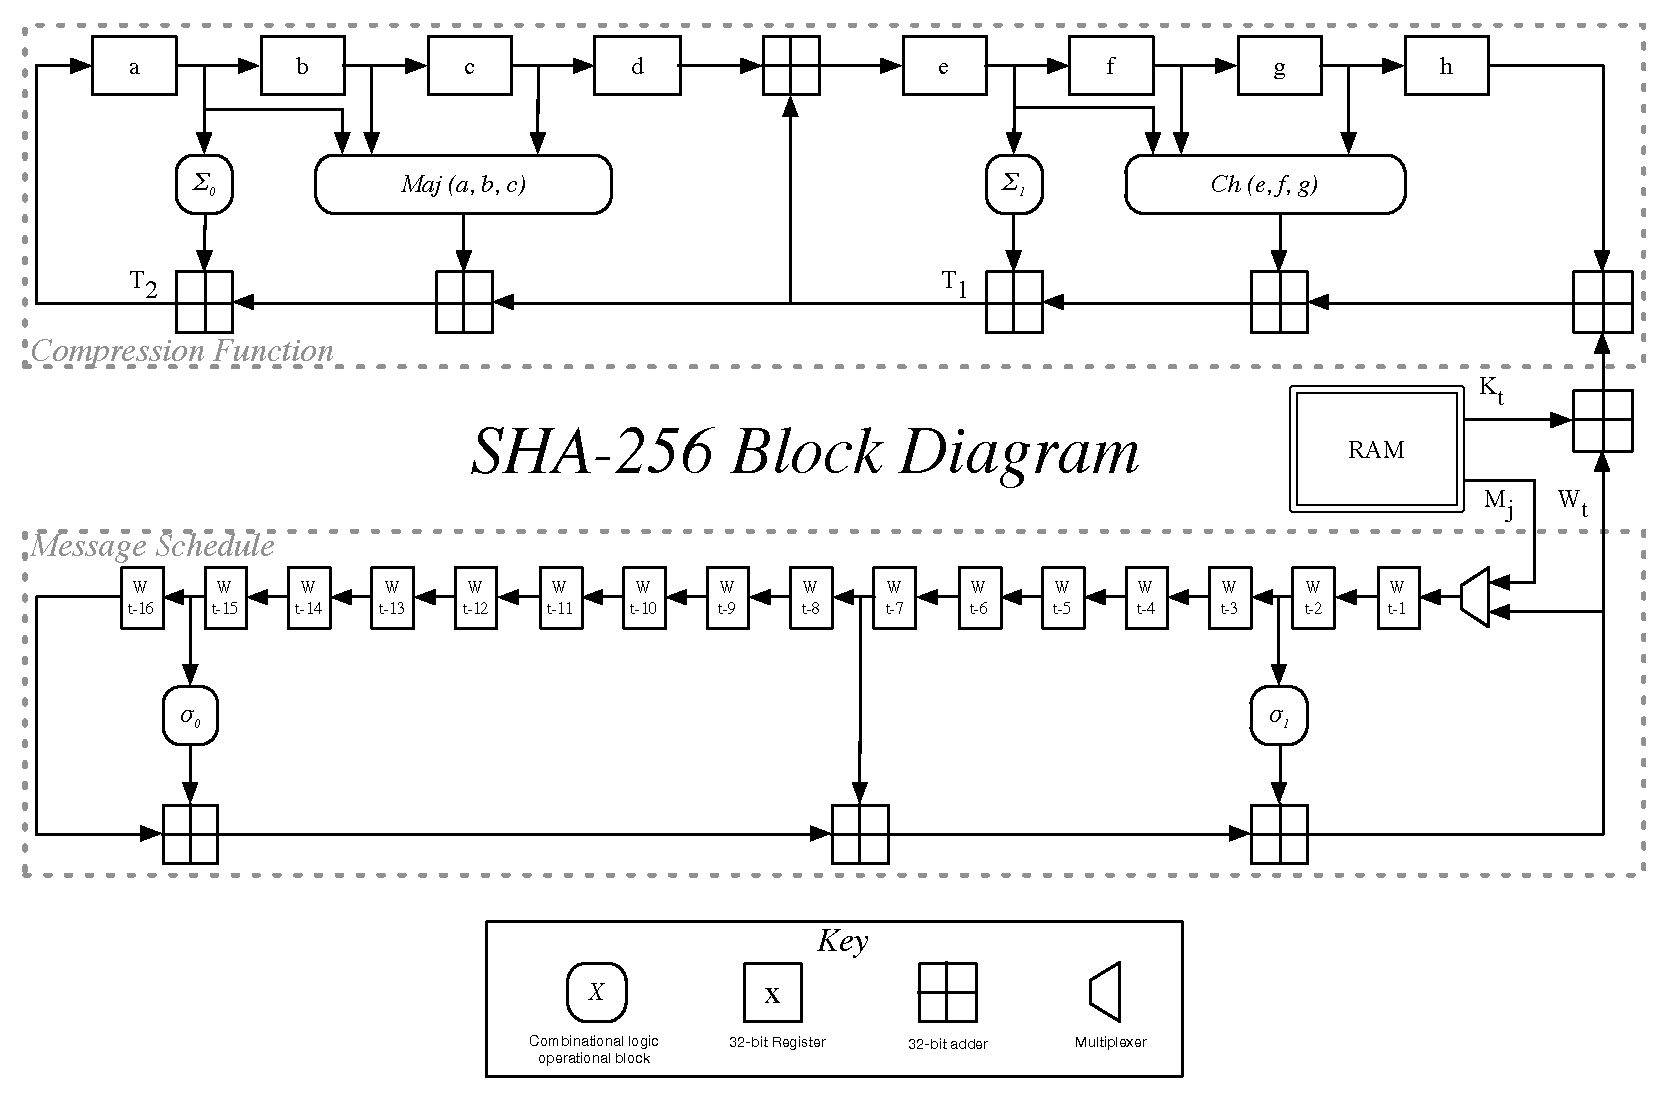
\includegraphics[angle=270, scale=0.7]{images/sha256}
  \caption{SHA-256 Block Diagram}
\end{figure}

\subsection{Implementation}

The internal implementation of a hash function can take many forms, however in
our case it must be through the use of linear feedback shift registers (LFSR)
throughout the design.

\section{True Random Number Generation on FPGA}
In Electronics a hardware clock is created from a harmonic oscillator such as a
quartz crystal whose output flips high to low and back at a regular interval.
The basics of the implementation of a random number generator to be used by the
fuzzy extractor is by sampling the output state of one hardware clock at times
controlled by another. We can utilise the clock drift as a source of randomness.
The two clocks are required to originate from two independent clock crystals
(one cannot be the Phased Locked Loop result of the other). Since a clocks
crystals are not perfectly precise in their oscillation due to thermal noise
effects ageing and variances in supply current and voltage it can be seen to be
unknown at a given time whether two independent clocks are in phase or not. 

If the frequency of one clock is very much higher than the other (1000s of
times), it can be seen as a type of digitised noise source in respect to the
readings that will be obtained at the sampling frequency imposed by the slower
clock.
However this implies that the bit rate of the output of the random number
generator will have to be very much lower than the fastest clock.
For the purposes of the Generation procedure in a Fuzzy extractor that is used
only once in a factory setting this issue may well not be a problem.
In reference to the implementation used the two random number generators used
need only to generate a few hundred bits of random data for each
Challenge//Response Pair.
Given that each generation procedure also required many clock cycles of activity
for BCH encoding and SHA-256 Hashing it would be possible to generate random
data of required length in the time it takes to complete a response.
However this random data is required at the start of the generation process,
therefore it would be expedient to generate the randomness required for the
first Fuzzy Extractor Generation Process during the devices initialisation
routines and store the result in a buffer. Then on subsequent generation
procedures, after the buffer contents has been accessed the random data
generation process can function in parallel, filling the buffer with new
randomness.

\section{Modified Ethernet Authentication Protocol Design}